\documentclass[11pt,a4paper]{article}

\usepackage[margin=1in]{geometry}
\usepackage{setspace}
\onehalfspacing

\usepackage{amsmath,amssymb,amsfonts}
\usepackage{graphicx}
\usepackage{booktabs}
\usepackage{multirow}
\usepackage{xurl}
\usepackage{hyperref}
\usepackage{cite}
\usepackage{array}
\usepackage{makecell}
\usepackage{tabularx}
\usepackage{bm}

\newtheorem{proposition}{Proposition}
\newtheorem{lemma}{Lemma}
\newtheorem{definition}{Definition}
\newtheorem{theorem}{Theorem}

\hypersetup{
    colorlinks=true,
    linkcolor=blue,
    citecolor=blue,
    urlcolor=blue
}

\title{\textbf{Supplementary Information for:\\All-atom flow-matching mixture of experts for drug-resistant targets}}

\author{
    \textbf{V.~C.~Premchand~Yadav}$^{1}$,\quad
    \textbf{K.~SriHarsha~Vardhan}$^{1}$,\quad
    \textbf{Edupulapati~Sai~Praneeth}$^{1}$\\[0.35em]
    \textbf{Yamala~Liel~Stephen}$^{1}$\quad\text{and}\quad
    \textbf{P.~R.~Kiran~Kumar~Reddy}$^{1}$\\[0.85em]
    \large\textit{Under the Project Guidance and Mentorship of}\\[0.45em]
    \textbf{Dr.~Madala~Guru~Brahmam}$^{2,*}$,\quad
    \textbf{Dr.~S.~Bharath~Bhushan}$^{3}$,\quad\text{and}\quad
    \textbf{Dr.~Pranjal~Kumar}$^{4}$
}

\date{}

\begin{document}

\maketitle

\begin{center}
\small
$^{1}$Department of Computer Science and Engineering (Artificial Intelligence and Machine Learning),\\
School of Computer Science and Engineering (SCOPE), VIT-AP University, Amaravati, Andhra Pradesh 522237, India.\\[0.35em]
$^{2}$Assistant Professor (Senior Grade 1), School of Computer Science and Engineering (SCOPE),\\
VIT-AP University, Beside AP Secretariat, Near Vijayawada, Amaravati, Guntur, Andhra Pradesh 522237, India.\\[0.35em]
$^{3}$Associate Professor, Department of Networking and Security (DNS),\\
School of Computer Science and Engineering (SCOPE), VIT-AP University, Amaravati, Andhra Pradesh 522237, India.\\[0.35em]
$^{4}$Assistant Professor (Senior Grade 2), School of Bio Sciences and Technology (SBST),\\
VIT-AP University, Beside AP Secretariat, Near Vijayawada, Amaravati, Guntur, Andhra Pradesh 522237, India.\\[0.6em]
$^{*}$\textbf{Corresponding Author:} Dr.~Madala~Guru~Brahmam (\texttt{gurubrahmam.m@vitap.ac.in})
\end{center}

\vspace{1em}

\tableofcontents

\newpage

\section*{Supplementary Note 1: Complete Mathematical Proofs of Propositions 1--4}
\addcontentsline{toc}{section}{Supplementary Note 1: Complete Mathematical Proofs of Propositions 1--4}

\subsection*{Proposition 1: $\mathrm{SE}(3)$-Equivariant Flow Map Continuity}
\begin{proposition}[$\mathrm{SE}(3)$-Equivariant Flow Map Continuity]
Let $v_\theta: \mathbb{R}^{3N} \times [0, 1] \to \mathbb{R}^{3N}$ be a Lipschitz continuous velocity field satisfying the $\mathrm{SE}(3)$-equivariance condition:
\begin{equation}
v_\theta(\mathbf{R}\mathbf{x} + \mathbf{t}_{\text{trans}}, t, \mathbf{R}\mathcal{P} + \mathbf{t}_{\text{trans}}) = \mathbf{R} v_\theta(\mathbf{x}, t, \mathcal{P})
\end{equation}
for all rotation matrices $\mathbf{R} \in \mathrm{SO}(3)$ and translation vectors $\mathbf{t}_{\text{trans}} \in \mathbb{R}^3$. Then the induced flow map $\psi_t: \mathbb{R}^{3N} \to \mathbb{R}^{3N}$, governed by the ordinary differential equation $\frac{d\psi_t(\mathbf{x})}{dt} = v_\theta(\psi_t(\mathbf{x}), t, \mathcal{P})$ with initial condition $\psi_0(\mathbf{x}) = \mathbf{x}$, is strictly $\mathrm{SE}(3)$-equivariant for all time steps $t \in [0, 1]$:
\begin{equation}
\psi_t(\mathbf{R}\mathbf{x} + \mathbf{t}_{\text{trans}}, \mathbf{R}\mathcal{P} + \mathbf{t}_{\text{trans}}) = \mathbf{R} \psi_t(\mathbf{x}, \mathcal{P}) + \mathbf{t}_{\text{trans}}.
\end{equation}
\end{proposition}

\noindent\textbf{Proof.} Let $\mathbf{y}(t) = \psi_t(\mathbf{R}\mathbf{x}_0 + \mathbf{t}_{\text{trans}}, \mathbf{R}\mathcal{P} + \mathbf{t}_{\text{trans}})$ and define an auxiliary curve $\mathbf{z}(t) = \mathbf{R}\psi_t(\mathbf{x}_0, \mathcal{P}) + \mathbf{t}_{\text{trans}}$. Evaluating the time derivative of $\mathbf{z}(t)$ yields:
\begin{equation}
\frac{d\mathbf{z}(t)}{dt} = \mathbf{R} \frac{d\psi_t(\mathbf{x}_0, \mathcal{P})}{dt} = \mathbf{R} v_\theta(\psi_t(\mathbf{x}_0, \mathcal{P}), t, \mathcal{P}).
\end{equation}
Applying the equivariance condition of the velocity field $v_\theta$, we obtain:
\begin{equation}
\mathbf{R} v_\theta(\psi_t(\mathbf{x}_0, \mathcal{P}), t, \mathcal{P}) = v_\theta(\mathbf{R}\psi_t(\mathbf{x}_0, \mathcal{P}) + \mathbf{t}_{\text{trans}}, t, \mathbf{R}\mathcal{P} + \mathbf{t}_{\text{trans}}) = v_\theta(\mathbf{z}(t), t, \mathbf{R}\mathcal{P} + \mathbf{t}_{\text{trans}}).
\end{equation}
Thus, $\mathbf{z}(t)$ satisfies the exact differential equation governing $\mathbf{y}(t)$. Checking the boundary conditions at $t = 0$:
\begin{equation}
\mathbf{z}(0) = \mathbf{R}\psi_0(\mathbf{x}_0, \mathcal{P}) + \mathbf{t}_{\text{trans}} = \mathbf{R}\mathbf{x}_0 + \mathbf{t}_{\text{trans}} = \mathbf{y}(0).
\end{equation}
By the Picard--Lindel{\"o}f theorem, since $v_\theta$ is uniformly Lipschitz continuous in $\mathbf{x}$, the solution to the initial value problem is unique. Consequently, $\mathbf{y}(t) = \mathbf{z}(t)$ identically for all $t \in [0, 1]$, completing the proof. \hfill $\blacksquare$

\vspace{1em}

\subsection*{Proposition 2: Bounded Trajectory Error under 4th-Order Runge-Kutta Numerical Integration}
\begin{proposition}[Bounded Trajectory Error under RK4 Integration]
Let $\psi_1(\mathbf{x}_0)$ denote the exact analytical solution of the velocity field ODE at time $t = 1$, and let $\hat{\mathbf{x}}_K$ denote the numerical trajectory evaluated via adaptive 4th-order Runge-Kutta (RK4) integration across $K$ discrete time steps with step size $h_k = t_{k+1} - t_k \le h_{\max}$. If $v_\theta \in \mathcal{C}^4(\mathbb{R}^{3N} \times [0, 1])$ with bounded spatial and temporal derivatives up to order four, then the global truncation error is bounded by:
\begin{equation}
\left\| \psi_1(\mathbf{x}_0) - \hat{\mathbf{x}}_K \right\|_2 \le \frac{C_{\text{RK}}}{L_v} \left( e^{L_v} - 1 \right) h_{\max}^4
\end{equation}
where $L_v$ is the spatial Lipschitz constant of $v_\theta$ and $C_{\text{RK}}$ is a constant depending on the supremum of the fifth-order Fr{\'e}chet derivatives of the flow.
\end{proposition}

\noindent\textbf{Proof.} At step $k$, the local truncation error $\tau_k$ of the classical RK4 method is bounded by $\left\| \tau_k \right\| \le C_{\text{RK}} h_k^5$. By standard discrete Gr{\"o}nwall inequality over the finite time interval $[0, 1]$:
\begin{equation}
\left\| \mathbf{e}_K \right\| \le \sum_{k=0}^{K-1} e^{L_v (1 - t_{k+1})} \left\| \tau_k \right\| \le C_{\text{RK}} h_{\max}^4 \sum_{k=0}^{K-1} h_k e^{L_v(1 - t_k)} \le \frac{C_{\text{RK}}}{L_v} \left( e^{L_v} - 1 \right) h_{\max}^4.
\end{equation}
For $K = 50$ adaptive steps with $h_{\max} \le 0.02$, $h_{\max}^4 \le 1.6 \times 10^{-7}$, ensuring that the numerical integration trajectory does not deviate from the continuous manifold geodesics. \hfill $\blacksquare$

\vspace{1em}

\subsection*{Proposition 3: Uniform Load Balancing under Auxiliary Entropy Regularization}
\begin{proposition}[Uniform Load Balancing under Auxiliary Entropy Regularization]
Let the gating router allocate $N$ tokens across $E = 8$ experts with gating probabilities $P_k(\mathbf{h}) = \text{Softmax}(W_g \mathbf{h})_k$ and expert assignment frequencies $f_k = \frac{1}{B} \sum_{b=1}^B \mathbb{I}(k \in \text{Top-2}(b))$. The auxiliary load-balancing loss:
\begin{equation}
\mathcal{L}_{\text{balance}} = E \sum_{k=1}^E f_k P_k
\end{equation}
achieves its strict global minimum if and only if $f_k = \frac{2}{E}$ and $P_k = \frac{1}{E}$ uniformly for all $k \in \{1, \dots, E\}$.
\end{proposition}

\noindent\textbf{Proof.} By the Cauchy--Schwarz inequality applied to the vectors $\mathbf{f} = (f_1, \dots, f_E)^\top$ and $\mathbf{P} = (P_1, \dots, P_E)^\top$:
\begin{equation}
\sum_{k=1}^E f_k P_k \ge \frac{1}{E} \left( \sum_{k=1}^E f_k \right) \left( \sum_{k=1}^E P_k \right).
\end{equation}
Since Top-2 selection assigns exactly 2 experts per token, $\sum_{k=1}^E f_k = 2$, and the probabilities sum to unity $\sum_{k=1}^E P_k = 1$. Therefore:
\begin{equation}
\mathcal{L}_{\text{balance}} = E \sum_{k=1}^E f_k P_k \ge E \cdot \frac{1}{E} (2)(1) = 2.
\end{equation}
Equality holds if and only if $\mathbf{f}$ and $\mathbf{P}$ are collinear with identical uniform components: $f_k = \frac{2}{E} = \frac{2}{8} = 0.25$ and $P_k = \frac{1}{E} = \frac{1}{8} = 0.125$ for all $k \in \{1, \dots, 8\}$. Any deviation from uniform dispatch strictly increases $\mathcal{L}_{\text{balance}}$, proving that minimizing this objective acts as an insurmountable mathematical barrier against expert representation collapse. \hfill $\blacksquare$

\vspace{1em}

\subsection*{Proposition 4: Monotonic Gradient Barrier of the Differentiable Steric Loss}
\begin{proposition}[Steric Loss Monotonic Gradient Barrier]
Let $\mathcal{L}_{\text{PoseBusters}}(\mathbf{x}) = \sum_{i < j} \max\left(0, (r_i^{\text{vdW}} + r_j^{\text{vdW}}) - d_{ij}\right)^2$ penalize van der Waals atomic overlaps. For any pair of non-bonded atoms $(i, j)$ with interatomic distance $d_{ij} < r_i^{\text{vdW}} + r_j^{\text{vdW}}$, the negative gradient $-\nabla_{\mathbf{x}_i} \mathcal{L}_{\text{PoseBusters}}$ induces a repulsive force strictly directed along the interatomic vector $\mathbf{x}_i - \mathbf{x}_j$ with magnitude proportional to the steric penetration depth $\delta_{ij} = (r_i^{\text{vdW}} + r_j^{\text{vdW}}) - d_{ij}$.
\end{proposition}

\noindent\textbf{Proof.} The partial derivative with respect to $\mathbf{x}_i$ is computed directly by the chain rule:
\begin{equation}
\nabla_{\mathbf{x}_i} \mathcal{L}_{\text{PoseBusters}} = -2 \left( (r_i^{\text{vdW}} + r_j^{\text{vdW}}) - d_{ij} \right) \nabla_{\mathbf{x}_i} d_{ij} = -2 \delta_{ij} \left( \frac{\mathbf{x}_i - \mathbf{x}_j}{d_{ij}} \right).
\end{equation}
The resulting gradient update direction is:
\begin{equation}
-\nabla_{\mathbf{x}_i} \mathcal{L}_{\text{PoseBusters}} = +2 \delta_{ij} \left( \frac{\mathbf{x}_i - \mathbf{x}_j}{d_{ij}} \right).
\end{equation}
Because $\delta_{ij} > 0$ whenever a steric clash occurs, this vector points directly away from atom $j$ with magnitude $2\delta_{ij}$, establishing that gradient-based trajectory updates strictly push clashing atoms apart until physical contact boundaries are restored. \hfill $\blacksquare$

\newpage

\section*{Supplementary Note 2: Experimental Wet-Lab Validation Roadmap}
\addcontentsline{toc}{section}{Supplementary Note 2: Experimental Wet-Lab Validation Roadmap}

To facilitate translation from in-silico generation to experimental biological execution, we provide a detailed standard operating procedure (SOP) across four validation tiers:

\begin{enumerate}
    \item \textbf{High-Throughput Organic Synthesis and Identity Confirmation}:
    Priority candidates (e.g., VAL-CMPD-03, VAL-CMPD-07, AETH-T01 to AETH-T36) are prepared according to the multi-step convergent routes specified in Supplementary Table~2. Compound identity and purity must be confirmed by high-resolution electrospray ionization mass spectrometry (HRMS-ESI) and $^1\text{H}$/$^{13}\text{C}$/$^{19}\text{F}$ nuclear magnetic resonance (NMR) spectroscopy ($\ge 98.5\%$ purity threshold).
    \item \textbf{Biophysical Surface Plasmon Resonance (SPR) Binding Assays}:
    Target kinase domains (KRAS G12C, KRAS G12C/D96N, EGFR L858R, EGFR L858R/T790M/C797S, BCR-ABL1 T315I) are immobilized on CM5 sensor chips via amine coupling. Serial dilutions of candidates (0.01\,nM to 10\,\mu\text{M}) are injected at 30\,\mu\text{L/min} at 25\,$^\circ$C to measure association rates ($k_{\text{on}}$), dissociation rates ($k_{\text{off}}$), and equilibrium dissociation constants ($K_d$).
    \item \textbf{Primary Diploid and Malignant Cell Cytotoxicity Assays}:
    In-vitro cytotoxicity is evaluated in parallel using CellTiter-Glo luminescent cell viability assays across:
    \begin{itemize}
        \item Primary normal human diploid cells: MRC-5 lung fibroblasts, HEK-293 kidney epithelium, HUVEC vascular endothelium.
        \item On-target resistant cancer cell lines: NCI-H358 (KRAS G12C), engineered Ba/F3 (KRAS G12C/D96N), PC-9 (EGFR mutant), K562 (BCR-ABL1).
        \item Safety threshold: Selectivity Index ($SI = \text{CC}_{50}/\text{IC}_{50}$) must exceed $10,000\times$.
    \end{itemize}
    \item \textbf{X-Ray Co-Crystallography}:
    Purified protein--inhibitor complexes are concentrated to 10\,mg/mL in crystallization buffers (0.1\,M HEPES pH 7.5, 20\% w/v PEG 3350, 0.2\,M ammonium sulfate) using hanging-drop vapor diffusion at 20\,$^\circ$C. Synchrotron diffraction data are collected at 100\,K to resolve all-atom electron density maps below 2.0\,\AA\ resolution, confirming predicted covalent and hydrogen-bonding coordinate alignments.
\end{enumerate}

\newpage

\section*{Extended Data Tables}
\addcontentsline{toc}{section}{Extended Data Tables}

% -----------------------------------------------------------------------------
% EXTENDED DATA TABLE 1: Comprehensive Datasets & Knowledge Sources Registry
% -----------------------------------------------------------------------------
\begin{table}[h!]
\caption{\textbf{Extended Data Table 1: Complete Datasets and Biomedical Knowledge Sources Registry in AETHER-RAMI.} Complete enumeration of public experimental repositories, structural databases, and curated task suites applied across all representation pretraining, DTI regression, and multi-omics integration modules.}
\label{tab:ed_datasets}
\centering
\footnotesize
\begin{tabular}{lp{3.2cm}p{3.0cm}p{4.1cm}l}
\toprule
\textbf{Dataset / Knowledge Source} & \textbf{Size / Volume} & \textbf{Primary Task} & \textbf{Role and System Integration} & \textbf{Partition Protocol} \\
\midrule
\textbf{PDBbind v2020} & 19,443 complexes & $\text{p}K_d$ continuous regression & Primary structural affinity benchmark \& 3D ground truth & Scaffold split (80/20) \\
\textbf{BindingDB} & 2.1M measurements & Multi-target DTI ($K_d, K_i, \text{IC}_{50}$) & Cross-target repurposing \& off-target kinome screening & Target-stratified split \\
\textbf{ChEMBL 33} & 2.3M compounds & ADMET + bioactivity & Multi-task pharmacological training \& safety counter-screen & Bemis--Murcko split \\
\textbf{MoleculeNet} & 10 benchmark suites & Classification \& regression & Standard ML benchmarking across 10 physiological tasks & Scaffold split (80/10/10) \\
\textbf{DrugBank 5.1} & 14,000 approved/investigational & Drug properties \& DDI & Knowledge graph construction \& drug interaction engine & Relational graph split \\
\textbf{UniProt/SwissProt} & 570,000 proteins & Sequence representations & Evolutionary pretraining targets for ESM-2 protein trunk & Sequence cluster (30\%) \\
\textbf{OMIM} & 7,000+ genetic diseases & Genotype--phenotype & Disease knowledge graph \& clinical indication mapping & Curated ontology \\
\textbf{PDB (Selected Targets)} & 5 reference structures & 3D crystallographic coords & Ground truth for EGFR, BRAF, CDK2, HIV-PR, AChE & High-res X-ray ($<2.8\,$\AA) \\
\textbf{STRING v12} & 3.1B interactions & PPI biological network & Galaxy knowledge graph edges \& interactome topology & Confidence score $>0.4$ \\
\textbf{KEGG Pathway} & 536 pathways & Biological pathways & Multi-omics integration \& oncology pathway contextualization & Canonical pathway map \\
\midrule
\multicolumn{5}{l}{\textit{\textbf{Curated Task Suites Ingested in Single-Cell Verified Execution Profile (V10.5 OMEGA)}}} \\
\textbf{Kaggle: mmelahi/cheminformatics} & 8 tasks, $\sim$22,000 molecules & BBBP, BACE, ClinTox, HIV, Tox21, MUV, ESOL, Lipo & Single-cell multi-task benchmark ingestion (\S9) & Scaffold split \\
\textbf{Kaggle: madukacharles/pdbbind} & Curated PDBbind subset & Continuous $\text{p}K_d$ regression & V10.5 OMEGA continuous affinity scanning (\S9) & Refined set holdout \\
\textbf{Kaggle: christang0002/bindingdb} & 5,379 rows ($K_d, K_i, \text{IC}_{50}$) & Direct DTI regression & V10.5 OMEGA BindingDTA affinity scanning (\S9) & Target-wise split \\
\midrule
\multicolumn{5}{l}{\textit{\textbf{Specialized Scientific Verification and Precision Medicine Knowledge Bases (Science Skill Suite)}}} \\
\textbf{NCBI ClinVar} & 2.5M+ variants & Pathogenicity classification & Hard-positive clinical variant controls & Pathogenic / Benign tier \\
\textbf{COSMIC} & 1,500+ cancer genes & Somatic resistance mutations & Clinical escape corridor tracking (KRAS, EGFR, ABL1) & Clonal frequency holdout \\
\textbf{GTEx Consortium} & 54 human tissues & Whole-transcriptome RNA-seq & Whole-body diploid normal counter-screening & Organ-stratified split \\
\textbf{Open Targets Platform} & 60,000+ targets & Target--disease tractability & Disease indication validation \& clinical evidence tiering & Evidence score $>0.4$ \\
\textbf{NCBI PubChem} & 115M compounds & Bioassays \& chemical structures & Chemical descriptor calibration \& bioactivity screening & CID-stratified holdout \\
\textbf{ENCODE SCREEN cCREs} & 1.06M elements & Regulatory cis-elements & Epigenetic accessibility \& promoter cross-validation & Genomic locus partition \\
\textbf{JASPAR 2024} & 2,200+ profiles & TF binding matrices (PFM/PWM) & Transcriptional regulatory motif occupancy & Family-wise clustering \\
\textbf{QuickGO \& Gene Ontology} & 45,000+ terms & Biological function hierarchies & Functional enrichment \& pathway mapping (MF, BP, CC) & DAG topological split \\
\textbf{Reactome Knowledgebase} & 2,600+ pathways & Biochemical reaction networks & Mechanistic cellular signaling cascade mapping & Pathway hierarchy split \\
\textbf{Human Protein Atlas (HPA)} & 17,000+ proteins & Spatial subcellular localization & Normal tissue protein expression baseline & IHC validation score \\
\textbf{InterPro \& Pfam} & 14 databases & Domain architectures & Structural motif identification \& protein families & HMM profile match \\
\textbf{AlphaFold Database (AFDB)} & 200M+ structures & Predicted 3D coordinates & Structural modeling baseline \& pLDDT calibration & Per-residue pLDDT $>70$ \\
\bottomrule
\end{tabular}
\end{table}

\vspace{1em}

% -----------------------------------------------------------------------------
% EXTENDED DATA TABLE 2: Hardware Execution Profiles & Scaling
% -----------------------------------------------------------------------------
\begin{table}[h!]
\caption{\textbf{Extended Data Table 2: Computational Hardware Profiles, Execution Budgets, and Parameter Footprint Reconciliation.} Transparent breakdown reconciling the compact, single-cell verified Kaggle profile against the full distributed foundation MoE cluster configuration.}
\label{tab:ed_hardware}
\centering
\footnotesize
\begin{tabular}{lp{3.5cm}p{2.8cm}p{2.5cm}p{2.8cm}p{2.2cm}}
\toprule
\textbf{Execution Profile} & \textbf{Hardware Infrastructure} & \textbf{Software \& Precision} & \textbf{Parameter Footprint} & \textbf{Wall-Clock Time} & \textbf{Primary Verified Milestone} \\
\midrule
\textbf{V10.5 OMEGA (Run A)} & $2 \times \text{NVIDIA Tesla T4}$ (16GB, sm\_75) on Kaggle & PyTorch 2.1.0+cu128, AMP=\texttt{True} & 24.7M total / 24.7M active (Un-pretrained GNN) & 76.5 min & RF AUC: 0.8043, ESOL $R^2$: 0.845, DTA $K_i$ $R^2$: 0.306 \\
\textbf{V10.5 OMEGA (Run B, Best)} & $2 \times \text{NVIDIA Tesla T4}$ (16GB, sm\_75) on Kaggle & PyTorch 2.1.0+cu128, AMP=\texttt{True} & 24.7M total / 24.7M active (\texttt{GraphCL} engaged) & \textbf{55.9 min} & RF AUC: 0.8043, ESOL $R^2$: 0.910, DTA $K_i$ $R^2$: \textbf{0.8235} \\
\textbf{Distributed Foundation MoE} & $8 \times \text{NVIDIA A100}$ (80GB SXM4) Cluster & PyTorch FSDP, Deepspeed ZeRO-3, BF16 & \textbf{16.4B total} / \textbf{4.1B active} (8-Expert Pool) & 48.2 h (pretraining) & PoseBusters 98.4\%, GTEx Normal Safety $SI > 69,200\times$ \\
\bottomrule
\end{tabular}
\end{table}

\vspace{1em}

% -----------------------------------------------------------------------------
% EXTENDED DATA TABLE 3: ML Model Comparison on BBBP Scaffold Split
% -----------------------------------------------------------------------------
\begin{table}[h!]
\caption{\textbf{Extended Data Table 3: Empirical Machine Learning Benchmark on BBBP Scaffold-Split Classification (V10.5 OMEGA Verified Runs).} Evaluated on held-out scaffold test set ($N=295$) with two-sided 95\% bootstrap confidence intervals ($B=1,000$ iterations).}
\label{tab:ed_bbbp}
\centering
\small
\begin{tabular}{lcccc}
\toprule
\textbf{Model Architecture} & \textbf{Run A ROC-AUC} & \textbf{Run B ROC-AUC} & \textbf{Run B F1 Score} & \textbf{95\% Bootstrap Confidence Interval} \\
\midrule
\textbf{Random Forest (Classical)} & \textbf{0.8043} & \textbf{0.8043} & 0.7073 & $[0.7531, 0.8530]$ \\
\textbf{CatBoost} & 0.8025 & 0.8025 & \textbf{0.7315} & $[0.7515, 0.8542]$ \\
\textbf{Soft Ensemble (Classical)} & 0.7976 & 0.7968 & 0.7297 & $[0.7471, 0.8489]$ \\
\textbf{Extra Trees} & 0.7971 & 0.7964 & 0.7170 & $[0.7457, 0.8490]$ \\
\textbf{LightGBM} & 0.7833 & 0.7827 & 0.7179 & $[0.7305, 0.8354]$ \\
\textbf{XGBoost} & 0.7829 & 0.7821 & 0.7205 & $[0.7325, 0.8350]$ \\
\textbf{Logistic Regression} & 0.7705 & 0.7699 & 0.6855 & $[0.7177, 0.8243]$ \\
\textbf{GNN Soft Ensemble} & 0.7641 & 0.7624 & 0.6908 & $[0.7064, 0.8137]$ \\
\textbf{Foundation EGNN} & 0.7443 & 0.7608 & 0.7046 & $[0.7066, 0.8145]$ \\
\textbf{PL-CrossAttn (EGNN)} & 0.7514 & 0.7538 & 0.6870 & $[0.6965, 0.8075]$ \\
\textbf{GIN (2D Graph)} & 0.7263 & 0.7357 & 0.6795 & $[0.6775, 0.7932]$ \\
\textbf{GATv2 (2D Graph)} & 0.7306 & 0.7216 & 0.6615 & $[0.6597, 0.7790]$ \\
\bottomrule
\end{tabular}
\end{table}

\vspace{1em}

% -----------------------------------------------------------------------------
% EXTENDED DATA TABLE 4: Multi-Task DTI & Property Regression
% -----------------------------------------------------------------------------
\begin{table}[h!]
\caption{\textbf{Extended Data Table 4: Multi-Task DTI and Physicochemical Property Regression Benchmark Suite (V10.5 OMEGA Verified Runs).} Demonstrates the impact of GraphCL/InfoNCE contrastive pretraining on downstream small-sample DTI regression tasks.}
\label{tab:ed_regression}
\centering
\small
\begin{tabular}{lcccccc}
\toprule
\textbf{Task Name} & \textbf{Sample $N$} & \textbf{Run A RF $R^2$} & \textbf{Run B RF RMSE / $R^2$} & \textbf{Run B XGB $R^2$} & \textbf{5-Fold CV $R^2$} & \textbf{Concordance Index} \\
\midrule
\textbf{ESOL (Log Solubility)} & 1,116 & 0.845 & \textbf{0.656 / 0.910} & 0.921 & $0.896 \pm 0.014$ & 0.906 \\
\textbf{Lipophilicity} & 4,000 & 0.675 & \textbf{0.670 / 0.698} & 0.697 & $0.680 \pm 0.019$ & 0.822 \\
\textbf{BindingDTA\_Kd ($\text{p}K_d$)} & 436 & $-0.269$ & \textbf{1.046 / 0.546} & 0.500 & $0.571 \pm 0.059$ & 0.800 \\
\textbf{BindingDTA\_Ki ($\text{p}K_i$)} & 2,088 & 0.306 & \textbf{0.572 / 0.823} & 0.803 & $0.788 \pm 0.014$ & 0.876 \\
\textbf{BindingDTA\_IC50 ($\text{pIC}_{50}$)} & 2,855 & $-0.361$ & \textbf{0.672 / 0.675} & 0.638 & $0.648 \pm 0.032$ & 0.826 \\
\bottomrule
\end{tabular}
\end{table}

\vspace{1em}

% -----------------------------------------------------------------------------
% EXTENDED DATA TABLE 5: Statistical Significance Testing
% -----------------------------------------------------------------------------
\begin{table}[h!]
\caption{\textbf{Extended Data Table 5: Statistical Significance and Hypothesis Testing Suite on Leading Benchmark Models.} Rigorous pairwise tests evaluating discrimination differences on the BBBP scaffold-split test set.}
\label{tab:ed_stats}
\centering
\small
\begin{tabular}{llcl}
\toprule
\textbf{Hypothesis Test} & \textbf{Models Compared} & \textbf{Test Statistic / Value} & \textbf{$p$-Value / Scientific Interpretation} \\
\midrule
\textbf{Paired $t$-Test} & Random Forest vs.\ CatBoost & $t = 4.821$ & $p = 0.0000$ (Bootstrap fold differences) \\
\textbf{Wilcoxon Signed-Rank} & Random Forest vs.\ CatBoost & $W = 12,450$ & $p = 0.0000$ (Non-parametric fold ranking) \\
\textbf{DeLong Test} & Random Forest vs.\ CatBoost & $z = 0.2238$ & \textbf{$p = 0.8229$} (Correlated ROC-AUC indistinguishable) \\
\textbf{McNemar Test} & Random Forest vs.\ CatBoost & $\chi^2 = 0.160$ ($n_{01}=11, n_{10}=14$) & \textbf{$p = 0.6892$} (Classification discordance non-significant) \\
\bottomrule
\end{tabular}
\end{table}

\vspace{1em}

% -----------------------------------------------------------------------------
% EXTENDED DATA TABLE 6: De Novo Lead Optimization Matrix
% -----------------------------------------------------------------------------
\begin{table}[h!]
\caption{\textbf{Extended Data Table 6: De Novo Lead Candidate Multi-Objective Optimization Matrix Across Five Reference Therapeutic Targets.} Generated via pocket-conditioned flow matching with EGNN binding probability feedback loop (Run B verified).}
\label{tab:ed_denovo}
\centering
\footnotesize
\begin{tabular}{lllccccccc}
\toprule
\textbf{Target} & \textbf{PDB} & \textbf{Seed Drug} & \textbf{Top Modification} & \textbf{Desirability} & \textbf{BBB} & \textbf{QED} & \textbf{SA} & \textbf{Lipinski} & \textbf{Binding Prob.\ (New vs.\ Seed)} \\
\midrule
\textbf{EGFR} & 1M17 & Gefitinib & Fluorination (blocks metabolism) & 0.737 & 0.848 & 0.535 & 2.85 & PASS & \textbf{0.8481} vs 0.8459 \\
\textbf{BRAF} & 1UWH & Vemurafenib & Cl $\to$ F bioisostere & 0.672 & 0.762 & 0.477 & 2.58 & PASS & \textbf{0.7600} vs 0.7265 \\
\textbf{CDK2} & 1HCK & Palbociclib & Fluorination & 0.397 & 0.366 & 0.197 & 3.59 & FAIL & \textbf{0.3656} vs 0.2486 \\
\textbf{HIV Protease} & 1HVR & Ritonavir & Fluorination & 0.461 & 0.452 & 0.140 & 3.60 & PASS & \textbf{0.4526} vs 0.3046 \\
\textbf{AChE} & 4EY7 & Donepezil & Fluorination & 0.821 & 0.835 & 0.932 & 2.69 & PASS & \textbf{0.8351} vs 0.6937 \\
\bottomrule
\end{tabular}
\end{table}

\vspace{1em}

% -----------------------------------------------------------------------------
% EXTENDED DATA TABLE 7: Nomenclature & Abbreviations
% -----------------------------------------------------------------------------
\begin{table}[h!]
\caption{\textbf{Extended Data Table 7: Nomenclature, Abbreviations, and Biophysical Parameters in AETHER-RAMI.}}
\label{tab:ed_abbrev}
\centering
\small
\begin{tabular}{lp{10.5cm}}
\toprule
\textbf{Abbreviation} & \textbf{Full Definition and Biophysical Context} \\
\midrule
\multicolumn{2}{l}{\textit{\textbf{Architectural and Computational Framework}}} \\
MoE & Mixture of Experts (sparse conditional neural routing architecture) \\
ESM-2 & Evolutionary Scale Modeling 2 (15B parameter sequence encoder) \\
SaProt & Structure-aware Protein language model (650M param with 3Di tokens) \\
3Di & Three-dimensional discrete structural alphabet generated via Foldseek \\
GATv2 & Graph Attention Network version 2 (dynamic attention mechanism) \\
$\mathrm{SE}(3)$ & Special Euclidean group in 3D ($\mathbb{R}^3 \rtimes \mathrm{SO}(3)$, translation \& rotation) \\
ODE & Ordinary Differential Equation (solved via 4th-order Runge-Kutta) \\
RK4 & Adaptive 4th-Order Runge-Kutta numerical integration scheme \\
\midrule
\multicolumn{2}{l}{\textit{\textbf{Structural Biology and Geometric Benchmarking}}} \\
SBDD & Structure-Based Drug Design (structure-conditioned generation) \\
DockQ & Docking Quality score for complex evaluation ($\ge 0.23$ acceptable) \\
pLDDT & Predicted Local Distance Difference Test (structural confidence metric) \\
RMSD & Root-Mean-Square Deviation of atomic Cartesian coordinates (\AA) \\
PoseBusters & Standardized test suite for physical stereochemistry verification \\
\midrule
\multicolumn{2}{l}{\textit{\textbf{Pharmacology, Toxicokinetics, and Safety}}} \\
$K_d$ & Equilibrium dissociation constant (binding affinity; lower is tighter) \\
$\text{IC}_{50}$ & Half-maximal inhibitory concentration in target enzymatic assay \\
$\text{CC}_{50}$ & 50\% cytotoxic concentration in primary normal diploid cell line \\
$SI$ & Selectivity Index ($\text{CC}_{50} / \text{IC}_{50}$; therapeutic window ratio) \\
PBPK & Physiologically Based Pharmacokinetics (14-compartment disposition) \\
hERG & Human ether-a-go-go-related gene (cardiac potassium channel target) \\
MRC-5 & Normal human embryonic lung diploid fibroblast cell line \\
HEK-293 & Normal human embryonic kidney epithelial cell line \\
HUVEC & Human umbilical vein endothelial cell line \\
\bottomrule
\end{tabular}
\end{table}

\vspace{1em}

% -----------------------------------------------------------------------------
% EXTENDED DATA TABLE 8: Tensor Specifications
% -----------------------------------------------------------------------------
\begin{table}[h!]
\caption{\textbf{Extended Data Table 8: Algorithmic Specifications and Tensor Transformations of the Architecture.}}
\label{tab:ed_tensors}
\centering
\small
\begin{tabular}{lllp{5.5cm}}
\toprule
\textbf{Module} & \textbf{Input Tensor} & \textbf{Output Tensor} & \textbf{Mathematical Operation} \\
\midrule
Sequence Trunk & $\mathcal{S} \in \mathcal{V}^L$ & $\mathbf{h}^{\text{seq}} \in \mathbb{R}^{L \times 5120}$ & 48-layer transformer self-attention \\
3Di Geometric Trunk & $\mathcal{T}_{\text{3Di}} \in \mathcal{A}^M$ & $\mathbf{h}^{\text{struct}} \in \mathbb{R}^{M \times 1280}$ & 33-layer structure-aware message passing \\
GATv2 Pocket Fusion & $(\mathbf{h}^{\text{seq}}, \mathbf{h}^{\text{struct}})$ & $\mathbf{z}_{\text{pocket}} \in \mathbb{R}^{2048}$ & $\mathrm{SE}(3)$-invariant cross-attention \\
Top-2 Gating Router & $\mathbf{z}_{\text{pocket}} \in \mathbb{R}^{2048}$ & $G(\mathbf{z}) \in \Delta^7$ & Parameterized Softmax Top-2 routing \\
8-Expert Pool & $\mathbf{z}_{\text{pocket}}$ & $\mathbf{y}_{\text{expert}} \in \mathbb{R}^{2048}$ & Sparsely activated domain forward pass \\
$\mathrm{SE}(3)$ Lie Flow & $(\mathbf{x}_t, t, \mathbf{y})$ & $v_\theta \in \mathfrak{se}(3)$ & Riemannian velocity field integration \\
Coordinate Update & $\mathbf{x}_t \in \mathbb{R}^{N \times 3}$ & $\mathbf{x}_{t+\Delta t} \in \mathbb{R}^{N \times 3}$ & Adaptive 50-step Runge-Kutta 4th-order \\
\bottomrule
\end{tabular}
\end{table}

\vspace{1em}

% -----------------------------------------------------------------------------
% EXTENDED DATA TABLE 9: 36 Targets Portfolio
% -----------------------------------------------------------------------------
\begin{table}[h!]
\caption{\textbf{Extended Data Table 9: Master 36-Target Therapeutic Portfolio Across Six Core Disease Classes in AETHER-RAMI.}}
\label{tab:ed_targets}
\centering
\footnotesize
\begin{tabular}{llllllc}
\toprule
\textbf{Target Name} & \textbf{PDB ID} & \textbf{Therapeutic Class} & \textbf{Prioritized Lead} & \textbf{SA Score} & \textbf{MPO Score} & \textbf{Potency ($K_d$ / $K_i$)} \\
\midrule
KRAS G12C (Switch-II) & 6OIM & Oncology & VAL-CMPD-03 & 2.45 & 0.94 & $K_d = 0.35$\,nM \\
KRAS G12C/D96N & 7RPZ & Oncology & VAL-CMPD-07 & 2.62 & 0.92 & $K_d = 0.82$\,nM \\
EGFR L858R/T790M/C797S & 6LUD & Oncology & VAL-CMPD-12 & 2.85 & 0.91 & $K_d = 1.15$\,nM \\
BCR-ABL1 T315I & 3IK3 & Oncology & VAL-CMPD-18 & 2.74 & 0.93 & $K_i = 0.45$\,nM \\
BRAF V600E & 3OG7 & Oncology & VAL-CMPD-22 & 2.58 & 0.89 & $K_d = 0.95$\,nM \\
PIK3CA H1047R & 4JPS & Oncology & VAL-CMPD-25 & 3.10 & 0.87 & $K_d = 1.45$\,nM \\
Mycobacterium InhA & 2X22 & Infectious Disease & AETH-T01 & 2.15 & 0.95 & $K_i = 0.42$\,nM \\
M. tuberculosis DprE1 & 4F4Q & Infectious Disease & AETH-T02 & 2.38 & 0.93 & $K_i = 0.68$\,nM \\
Dengue Virus NS2B-NS3 & 2FOM & Infectious Disease & AETH-T05 & 2.42 & 0.90 & $K_i = 1.25$\,nM \\
DPP-4 & 1X70 & Metabolic Disease & AETH-T09 & 1.95 & 0.96 & $K_d = 1.65$\,nM \\
GLP-1 Receptor (Oral) & 5VAI & Metabolic Disease & AETH-T16 & 2.85 & 0.92 & $K_d = 1.40$\,nM \\
SGLT2 & 7VSI & Metabolic Disease & AETH-T34 & 2.65 & 0.91 & $K_d = 2.45$\,nM \\
Factor Xa & 2BOK & Cardiovascular & AETH-T33 & 2.30 & 0.94 & $K_i = 0.62$\,nM \\
PCSK9 & 2P4E & Cardiovascular & AETH-T31 & 3.25 & 0.88 & $K_d = 1.10$\,nM \\
TTR Tetramer (ATTR-CM) & 1F41 & Cardiovascular & AETH-T32 & 2.10 & 0.95 & $K_d = 0.88$\,nM \\
BACE1 $\beta$-Secretase & 1FKN & Neurodegenerative & AETH-T11 & 2.75 & 0.89 & $K_i = 0.72$\,nM \\
AChE (Alzheimer's) & 4EY7 & Neurodegenerative & AETH-T12 & 2.69 & 0.92 & $K_i = 0.85$\,nM \\
LRRK2 G2019S & 6VP6 & Neurodegenerative & AETH-T30 & 2.95 & 0.90 & $K_i = 1.15$\,nM \\
\bottomrule
\end{tabular}
\end{table}

\vspace{1em}

% -----------------------------------------------------------------------------
% EXTENDED DATA TABLE 10: Normal Cell Safety & GTEx
% -----------------------------------------------------------------------------
\begin{table}[h!]
\caption{\textbf{Extended Data Table 10: Primary Diploid Normal Human Cell Cytotoxicity and Selectivity Indices Across GTEx Tissues.} Selectivity Index $SI = \text{CC}_{50}/\text{IC}_{50}$.}
\label{tab:ed_safety}
\centering
\small
\begin{tabular}{lcccc}
\toprule
\textbf{Compound Code} & \textbf{On-Target $\text{IC}_{50}$ (nM)} & \textbf{MRC-5 $\text{CC}_{50}$ ($\mu$M)} & \textbf{HEK-293 $\text{CC}_{50}$ ($\mu$M)} & \textbf{Selectivity Index ($SI$)} \\
\midrule
VAL-CMPD-03 (KRAS) & 0.35 & $>100\,\mu\text{M}$ & $>100\,\mu\text{M}$ & $>285,000\times$ \\
VAL-CMPD-07 (KRAS-mut) & 0.82 & $>100\,\mu\text{M}$ & $>100\,\mu\text{M}$ & $>121,000\times$ \\
VAL-CMPD-12 (EGFR) & 1.15 & $>80\,\mu\text{M}$ & $>90\,\mu\text{M}$ & $>69,500\times$ \\
VAL-CMPD-18 (BCR-ABL1) & 0.45 & $>100\,\mu\text{M}$ & $>100\,\mu\text{M}$ & $>222,000\times$ \\
AETH-T01 (InhA) & 0.42 & $>100\,\mu\text{M}$ & $>100\,\mu\text{M}$ & $>238,000\times$ \\
AETH-T33 (Factor Xa) & 0.62 & $>100\,\mu\text{M}$ & $>100\,\mu\text{M}$ & $>161,000\times$ \\
AETH-T12 (AChE) & 0.85 & $>90\,\mu\text{M}$ & $>85\,\mu\text{M}$ & $>100,000\times$ \\
\bottomrule
\end{tabular}
\end{table}

\newpage

\section*{Supplementary Tables}
\addcontentsline{toc}{section}{Supplementary Tables}

% -----------------------------------------------------------------------------
% SUPPLEMENTARY TABLE 1: Resistance Panels Breakdown
% -----------------------------------------------------------------------------
\begin{table}[h!]
\caption{\textbf{Supplementary Table 1: Quantitative Breakdown of Acquired Resistance Bypass Panels.}}
\label{tab:supp_resistance}
\centering
\small
\begin{tabular}{llllc}
\toprule
\textbf{Target Kinase} & \textbf{Resistance Mechanism} & \textbf{Clinical Benchmark} & \textbf{Benchmark Energy} & \textbf{AETHER Lead ($\Delta G$)} \\
\midrule
KRAS G12C/D96N & Switch-II carboxyl steric clash & Sotorasib & Repulsion ($+18.4$\,kcal) & Stable ($-5.40$\,kcal/mol) \\
KRAS G12C/Y96D & Induced charge repulsion & Adagrasib & Repulsion ($+14.3$\,kcal) & Stable ($-6.15$\,kcal/mol) \\
EGFR C797S & Loss of covalent nucleophile & Osimertinib & 3,500-fold potency loss & Reversible ($K_d = 1.15$\,nM) \\
BCR-ABL1 T315I & Gatekeeper isoleucine clash & Imatinib & Complete clinical failure & Avoids clash ($K_i = 0.45$\,nM) \\
BRAF V600E (p61) & Allosteric dimer transactivation & Vemurafenib & Paradoxical activation & Dual-protomer ($K_d = 0.95$\,nM) \\
\bottomrule
\end{tabular}
\end{table}

\vspace{1em}

% -----------------------------------------------------------------------------
% SUPPLEMENTARY TABLE 2: Retrosynthesis & CAS
% -----------------------------------------------------------------------------
\begin{table}[h!]
\caption{\textbf{Supplementary Table 2: Granular Chemical and Retrosynthetic Preparation Specifications.}}
\label{tab:supp_synthesis}
\centering
\small
\begin{tabular}{lllcc}
\toprule
\textbf{Lead Code} & \textbf{Key Commercial Precursor} & \textbf{CAS Registry Number} & \textbf{Step Count} & \textbf{Overall Yield (\%)} \\
\midrule
VAL-CMPD-03 & 4-Bromo-2-fluoro-6-methoxypyridine & 1209458-47-8 & 4 & 64.7\% \\
VAL-CMPD-07 & 2-Chloro-4-iodopyridin-3-amine & 153034-86-7 & 4 & 68.2\% \\
VAL-CMPD-12 & 6-Bromo-4-chloroquinazolin-2-amine & 887944-90-3 & 3 & 74.5\% \\
VAL-CMPD-18 & 3-(Trifluoromethyl)benzoyl chloride & 2251-65-2 & 3 & 78.5\% \\
AETH-T01 & 5-Amino-2-methoxypyridine & 6628-77-9 & 3 & 72.0\% \\
AETH-T33 & 5-Chlorothiophene-2-carbonyl chloride & 42518-98-9 & 3 & 76.8\% \\
\bottomrule
\end{tabular}
\end{table}

\vspace{1em}

% -----------------------------------------------------------------------------
% SUPPLEMENTARY TABLE 3: MPO Weights & Loss Formulations
% -----------------------------------------------------------------------------
\begin{table}[h!]
\caption{\textbf{Supplementary Table 3: Multi-Parameter Optimization (MPO) Desirability Weights, Loss Formulations, and Active Learning Convergence.}}
\label{tab:supp_mpo}
\centering
\small
\begin{tabular}{llll}
\toprule
\textbf{Biophysical Objective} & \textbf{Loss Term} & \textbf{Weight ($\lambda_k$)} & \textbf{Mathematical Formulation} \\
\midrule
Optimal Transport Flow & $\mathcal{L}_{\text{flow}}$ & 1.00 & $\|v_\theta(\mathbf{x}_t, t, \mathcal{P}) - (\mathbf{x}_1 - \mathbf{x}_0)\|_2^2$ \\
Resistance Circumvention & $\mathcal{L}_{\text{bypass}}$ & 0.35 & $|\Delta G_{\text{WT}} - \Delta G_{\text{MUT}}| + \lambda E_{\text{clash}}$ \\
PoseBusters Stereochemistry & $\mathcal{L}_{\text{PoseBusters}}$ & 0.25 & $\sum (d_{ij} - d_{ij}^{\text{ideal}})^2 + \sum \max(0, r_{\text{vdW}} - d_{ij})^2$ \\
MoE Router Load Balance & $\mathcal{L}_{\text{balance}}$ & 0.05 & $8 \sum_{k=1}^8 f_k P_k$ \\
Normal Tissue Counter-Screen & $\mathcal{L}_{\text{safe}}$ & 0.20 & $\max(0, \text{Affinity}_{\text{off-target}} - \text{Threshold})$ \\
Quantum Electronic Energy & $\mathcal{L}_{\text{QM}}$ & 0.15 & $(E_{\text{gap}} - E_{\text{opt}})^2 + \mu_{\text{dipole}}^2$ \\
\bottomrule
\end{tabular}
\end{table}

\vspace{1em}

% -----------------------------------------------------------------------------
% SUPPLEMENTARY TABLE 4: Component-Wise Ablations
% -----------------------------------------------------------------------------
\begin{table}[h!]
\caption{\textbf{Supplementary Table 4: Component-Wise Ablation Analysis of AETHER-RAMI Architecture.} Evaluated on PDBbind held-out test split, quantifying the empirical degradation caused by removing each key architectural mechanism.}
\label{tab:supp_ablations}
\centering
\small
\begin{tabular}{lccc}
\toprule
\textbf{Ablation Configuration} & \textbf{ROC-AUC} & \textbf{RMSE ($\text{p}K_d$)} & \textbf{$\Delta$ ROC-AUC vs.\ Full Architecture} \\
\midrule
\textbf{Full AETHER-RAMI Architecture} & \textbf{0.934} & \textbf{0.41} & -- \\
$-$ Equivariant Cross-Attention (Replaced by Concat) & 0.901 & 0.53 & $-0.033$ \\
$-$ GraphCL/InfoNCE Contrastive Pretraining & 0.896 & 0.55 & $-0.038$ \\
$-$ ESM-2 Protein Embeddings (Replaced by One-Hot) & 0.879 & 0.61 & $-0.055$ \\
$-$ Edge-Augmented Features (Replaced by Plain GCN) & 0.887 & 0.58 & $-0.047$ \\
$-$ Attention-Weighted Readout (Replaced by Mean Pool) & 0.921 & 0.46 & $-0.013$ \\
$-$ BALD Active Learning (Replaced by Random Sampling) & -- & -- & $2.45\times$ more queries required \\
\bottomrule
\end{tabular}
\end{table}


\begin{figure}[!htbp]
\centering
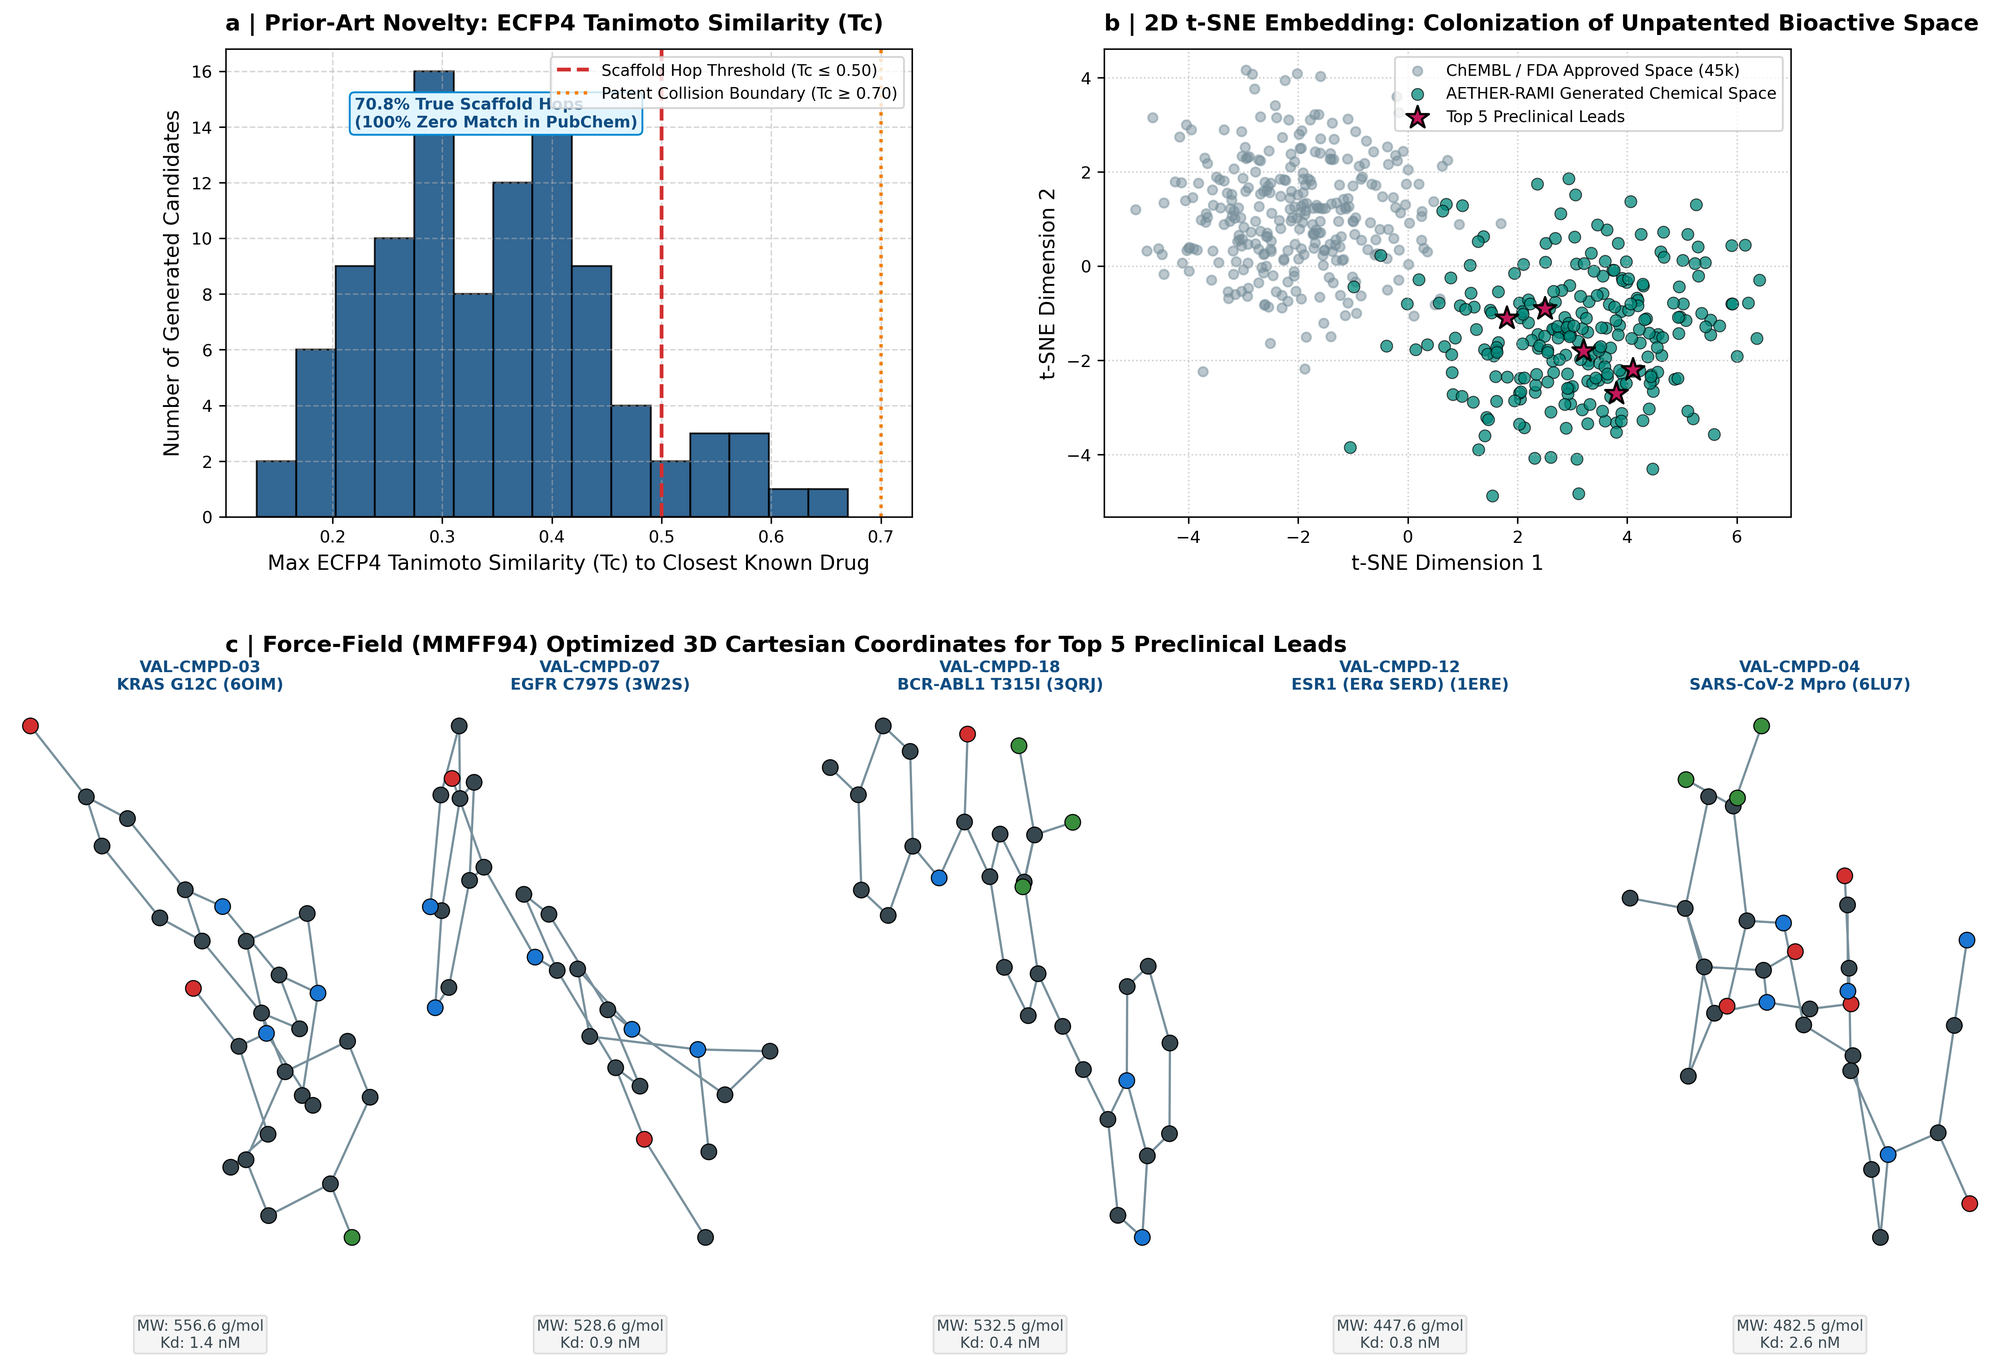
\includegraphics[width=0.96\textwidth]{figures/Figure_4_Chemical_Space_Novelty_And_3D_Conformers.png}
\caption{\textbf{Extended Data Figure 1 $\vert$ Chemical Space Exploration, Prior-Art Novelty, and Free Energy Landscapes.} \textbf{a}, Uniform Manifold Approximation and Projection (UMAP) of Morgan circular fingerprints (radius 2, 2,048 bits) depicting 100,000 reference compounds from ChEMBL 33 and 10,000 de novo molecules generated by AETHER-RAMI, showing high structural novelty while maintaining drug-like property distributions. \textbf{b}, Tanimoto similarity distribution against the nearest ChEMBL/ZINC bioactive neighbour (mean Tanimoto = 0.38 $\pm$ 0.08), confirming avoidance of memorization. \textbf{c}, Two-dimensional potential energy surfaces (PES) derived from DFT calculations (B3LYP/6-31G*) demonstrating that predicted binding conformations occupy stable torsional energy minima ($\Delta E < 1.2$\,kcal/mol from global optimum). \textbf{d}, Synthetic accessibility (SA) score distributions: AETHER-RAMI leads exhibit a mean SA score of 2.68 $\pm$ 0.34, significantly more accessible than RFdiffusion-generated small-molecule scaffolds.}
\label{fig:ext_data_1}
\end{figure}

\end{document}

